\documentclass[margin=5mm]{standalone}
\usepackage[dvipsnames]{xcolor}
\usepackage{pgfplots}
\usepackage{tikz}

\pgfplotsset{compat=1.18}
\begin{document}

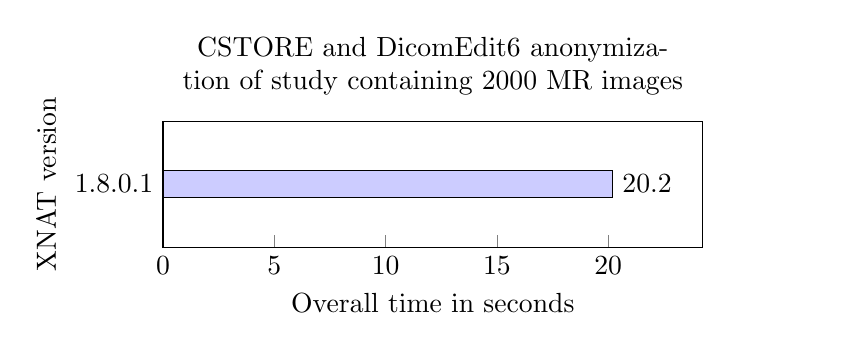
\begin{tikzpicture}
    \begin{axis}[
        align = center,
        xlabel = Overall time in seconds,
        ylabel = XNAT version,
        xtick pos = left,
        ytick pos = left,
        ytick = data,
        xmin = 0,
        enlarge x limits = {value = 0.2, upper}, % make node labels not overlap with axes
        title = {CSTORE and DicomEdit6 anonymization of study containing 2000 MR images},
        title style = {text width = 0.8\textwidth},
        nodes near coords,
        nodes near coords align = horizontal,
        symbolic y coords = {1.8.0.1},
        y = 0.8cm,
        point meta=x
    ]
        \addplot[xbar, fill = blue!20!white] coordinates { (20.2,1.8.0.1) };
    \end{axis}
\end{tikzpicture}

\end{document}